\documentclass{jlreq}

\usepackage{amsmath,amsthm,thmtools,amssymb}
\usepackage{tikz}
\usetikzlibrary{calc}

\allowdisplaybreaks[1]

\declaretheoremstyle[ %定理スタイル
spaceabove=\baselineskip,
headfont=\bfseries,
notefont=\bfseries,
headpunct=\relax,
postheadspace=\zw,
spacebelow=\baselineskip
]{thmsty}

\declaretheorem[ %定義環境
style=thmsty,
title=定義
]{definition}
\declaretheorem[ %定理環境
style=thmsty,
title=定理,
qed=\square
]{theorem}
\declaretheorem[ %系環境
style=thmsty,
title=系,
sibling=theorem,
qed=\square
]{corollary}
\declaretheorem[ %証明環境
style=thmsty,
title=証明,
numbered=no,
qed=\qedsymbol
]{myproof}
\renewenvironment{proof}{\begin{myproof}}{\end{myproof}}

\renewcommand{\qedsymbol}{$\blacksquare$} %墓石記号

\title{区分求積法}
\author{オ}
\date{\today}

\begin{document}
	
\maketitle

\begin{abstract}
	区分求積法について解説した.
\end{abstract}

\section{区分求積法の確認}

まずは,区分求積法の主張を確認しよう.

\begin{theorem}[区分求積法]\label{thm:quadrature_by_pts}
	$f(x)$を区間$[a,b]\ (a,b\in \mathbb{R},\,a\le b)$を上の連続関数
	\footnote{
		実際には,$f(x)$は区間$[a,b]$のほとんど至る所で連続であれば十分である.
	}
	とする.
	また,$\Delta_n=\dfrac{b-a}{n}$とおく.このとき,
	\begin{equation*}
		\lim_{n\to \infty}\sum_{k=0}^{n-1}f(a+k\Delta_n )\Delta_n=\int_{a}^{b}f(x)\,dx
	\end{equation*}
	が成り立つ.
\end{theorem}

もしかすると,定理\ref{thm:quadrature_by_pts}の形で区分求積法を使ったことはないかもしれない.
よく使われるのは,次の特別な場合であろう.

\begin{corollary}\label{cor:quadrature_by_pts}
	$f(x)$を区間$[0,1]$上で定義された関数とする.
	このとき,
	\begin{equation*}
		\lim_{n\to \infty}\frac{1}{n}\sum_{k=0}^{n-1}f\left(\frac{k}{n}\right)=\int_{0}^{1}f(x)\,dx
	\end{equation*}
	が成り立つ.
\end{corollary}

\begin{proof}
	定理\ref{thm:quadrature_by_pts}において,$a=0,\, b=1$とすればよい.
\end{proof}

実際には,系\ref{cor:quadrature_by_pts}の形を知っていれば十分である.
定理\ref{thm:quadrature_by_pts}の関数$f(x)$に対して,新しい関数$g(x)$を
\begin{equation*}
	g(x)=f(xb+(1-x)a)
\end{equation*}
で定めれば,$g(x)$は区間$[0,1]$で連続となる.
この$g(x)$に系\ref{cor:quadrature_by_pts}を適用すれば,定理$\ref{thm:quadrature_by_pts}$が得られる.

\section{区分求積法の意味}

区分求積法は,図形の面積を求める方法の一つに過ぎない.
今回は,そのことを確認することが目標である.

以下では,定理\ref{thm:quadrature_by_pts}での記号を用いる.
また,簡単のために,$f(x)$は区間$[a,b]$において非負であると仮定する.

$y=f(x)$のグラフと$x$軸及び直線$x=a,\ x=b$で囲まれた図形の面積を求めることを考える.
つまり,
\begin{equation*} %ここです
	\begin{tikzpicture}[baseline=40] %n=infty
		\newcommand{\A}{-1.7}
		\newcommand{\B}{1.3}
		\coordinate[label=below:$a$] (a) at (-1.7,0); %a
		\coordinate[label=below:$b$] (b) at (1.3,0); %b
		\filldraw[fill=lightgray] (a) -- plot[domain=\A:\B](\x,{(pow(\x,3)-3*\x)/3+2}) -- (b);
		\draw[->] (-2.7,0) -- (2.7,0) node[right]{$x$}; %x軸
		\draw[smooth,domain=-2.2:2.2] plot(\x, { (pow(\x,3)-3*\x)/3+2 }) node[above] {$y=f(x)$}; %f(x)
		\draw ($(\A,1)!0.5!(\B,1)$) node[fill=white] {ここ};
	\end{tikzpicture}
\end{equation*}
の面積を求めるのである.
この図形は上側がクネクネしていて,簡単には面積が求められなさそうに見える.
定積分を用いればすぐに求められるかもしれないが,ここでは,もっと素朴で,直感的な方法を考えよう.

この図形の面積が求めにくい理由は,上側がクネクネしているからに尽きる.
逆に言えば,クネクネさえしていなければ,面積は小学生でも求められるだろう.
そこで,この図形を,もっと単純な(クネクネしていない)形で近似してしてしまって,面積に近い値を求めてしまおうというのが,区分求積法の発想である.

まずは,次のように近似してみる.
\begin{equation*}
	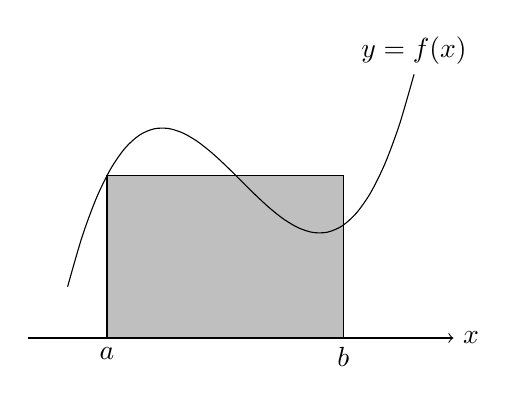
\begin{tikzpicture}[baseline=40] %n=1
		\newcommand{\n}{1}
		\newcommand{\A}{-1.7}
		\newcommand{\B}{1.3}
		\coordinate[label=below:$a$] (a) at (\A,0); %a
		\coordinate[label=below:$b$] (b) at (\B,0); %b
		\foreach \x in {0,...,0}{ %区分和
			\filldraw[fill=lightgray] ($(a)+{\x}*(${1/\n}*($(b)-(a)$)$)$)
			|- ($(a)+{\x+1}*(${1/\n}*($(b)-(a)$)$)+(0,{ (pow(\A+\x/\n*(\B-\A),3)-3*(\A+\x/\n*(\B-\A)))/3+2 })$)
			-- ($(a)+{\x+1}*(${1/\n}*($(b)-(a)$)$)$);
		}
		\draw[->] (-2.7,0) -- (2.7,0) node[right]{$x$}; %x軸
		\draw[smooth,domain=-2.2:2.2] plot(\x, { (pow(\x,3)-3*\x)/3+2 }) node[above] {$y=f(x)$}; %f(x)
	\end{tikzpicture}
\end{equation*}
つまり,幅$b-a$,高さ$f(a)$の長方形で,もとの図形を近似するのである.
この長方形の面積は
\begin{equation*}
	(b-a)f(a)
\end{equation*}
と簡単に求められるが,これはさすがに手を抜きすぎ
\footnote{
	平均値の定理より,高さをうまく調整すれば,この長方形の面積をもとの面積に一致させることができる.}
で,関数によっては全くあてにならないだろう.
そこで,区分求積法では,この長方形の数を増やして,どんどん近似の精度を良くしていく.

例えば,区間$[a,b]$を7等分して,それぞれの区間で今の近似を行ってみよう.
つまり,次の図のように,7つの長方形を用いて近似を行う.
\begin{equation*}
	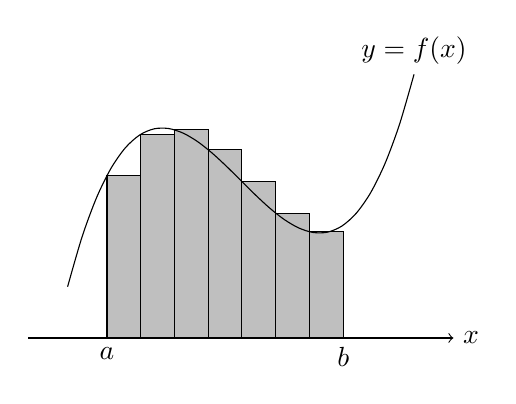
\begin{tikzpicture}[baseline=40] %n=7
		\newcommand{\n}{7}
		\newcommand{\A}{-1.7}
		\newcommand{\B}{1.3}
		\coordinate[label=below:$a$] (a) at (-1.7,0); %a
		\coordinate[label=below:$b$] (b) at (1.3,0); %b
		\foreach \x in {0,...,6}{ %区分和
			\filldraw[fill=lightgray] ($(a)+{\x}*(${1/\n}*($(b)-(a)$)$)$)
			|- ($(a)+{\x+1}*(${1/\n}*($(b)-(a)$)$)+(0,{ (pow(\A+\x/\n*(\B-\A),3)-3*(\A+\x/\n*(\B-\A)))/3+2 })$)
			-- ($(a)+{\x+1}*(${1/\n}*($(b)-(a)$)$)$);
		}
		\draw[->] (-2.7,0) -- (2.7,0) node[right]{$x$}; %x軸
		\draw[smooth,domain=-2.2:2.2] plot(\x, { (pow(\x,3)-3*\x)/3+2 }) node[above] {$y=f(x)$}; %f(x)
	\end{tikzpicture}
\end{equation*}
先ほどの1つの長方形を用いた近似と比べれば,よりいい感じにもとの図形を近似できていそうに見える.
この長方形たちの面積の合計を求めよう.

各長方形の幅は,区間$[a,b]$を7等分しているので
\begin{equation*}
	\Delta_7=\frac{b-a}{7}
\end{equation*}
だと分かる.
また,各長方形の高さは,左から順に
\begin{equation*}
	f(a),\quad f(a+\Delta_7), \quad f(a+2\Delta_7),\quad \dotsc,\quad f(a+6\Delta_7)
\end{equation*}
である
\footnote{
	今回は各小区間の左端における$f(x)$の値を高さにしたが,実は,高さは各小区間における$f(x)$の値域の中であれば好きなようにとれる.}.
これは,区間を7等分していることから分かる.
\begin{equation*}
	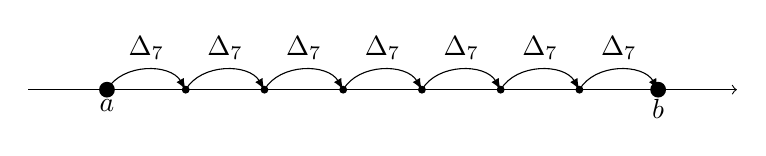
\begin{tikzpicture}
		\draw[->] (-1,0) -- (8,0);
		\fill (0,0) circle (0.1) node[below] {$a$}; 
		\fill (7,0) circle (0.1) node[below] {$b$};
		\foreach \x in {0,...,6}{
			\draw[bend left=60,-latex] (\x,0) to node[midway,above] {$\Delta_7$} (\x+1,0);
			\fill (\x+1,0) circle (0.05);
		}
	\end{tikzpicture}
\end{equation*}
よって,長方形たちの面積の合計は
\begin{equation*}
	\sum_{k=0}^{6}f(a+k\Delta_7)\Delta_7
\end{equation*}
である.

同様にして区間を30等分したとき,図形の近似は次のようになる.
\begin{equation*}
	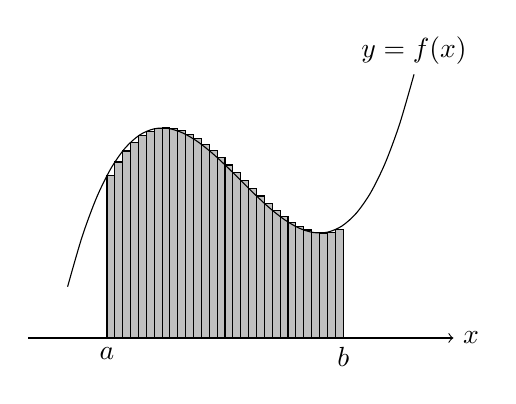
\begin{tikzpicture}[baseline=40] %n=30
		\newcommand{\n}{30}
		\newcommand{\A}{-1.7}
		\newcommand{\B}{1.3}
		\coordinate[label=below:$a$] (a) at (-1.7,0); %a
		\coordinate[label=below:$b$] (b) at (1.3,0); %b
		\foreach \x in {0,...,29}{ %区分和
			\filldraw[fill=lightgray] ($(a)+{\x}*(${1/\n}*($(b)-(a)$)$)$)
			|- ($(a)+{\x+1}*(${1/\n}*($(b)-(a)$)$)+(0,{ (pow(\A+\x/\n*(\B-\A),3)-3*(\A+\x/\n*(\B-\A)))/3+2 })$)
			-- ($(a)+{\x+1}*(${1/\n}*($(b)-(a)$)$)$);
		}
		\draw[->] (-2.7,0) -- (2.7,0) node[right]{$x$}; %x軸
		\draw[smooth,domain=-2.2:2.2] plot(\x, { (pow(\x,3)-3*\x)/3+2 }) node[above] {$y=f(x)$}; %f(x)
	\end{tikzpicture}
\end{equation*}
今までと比べれば,かなり精度が良くなっている.
このときの長方形たちの面積の合計も,先ほどと同様にすれば
\begin{equation*}
	\sum_{k=0}^{29}f(a+k\Delta_{30})\Delta_{30}
\end{equation*}
だと分かる.
図形がかなり良く近似できているので,この値も,もとの図形の面積にかなり近くなる.

以上のように,区間を細かく分割し,それぞれの小区間で長方形による近似を行えば,もとの図形の良い近似を得ることができる.
極限の考えを使えば,区間を限りなく細かく分割することで,もとの図形の面積を得られることが分かる.
よって,区間を$n$等分したとして,この$n$を無限大に発散させた極限値,つまり
\begin{equation*}
	\lim_{n\to \infty}\sum_{k=0}^{n-1}f(a+k\Delta_n )\Delta_n
\end{equation*}
が求めたかった面積となる
\footnote{
	実は,現代数学においては,この極限値(のより一般的な形)で定積分を定義する.
	多変数関数の積分である重積分や,複素数を値にもつ関数の積分である複素積分も同様にして定義される.}.
したがって,定理\ref{thm:quadrature_by_pts}が成り立つのである.
\begin{align*} %近似の図
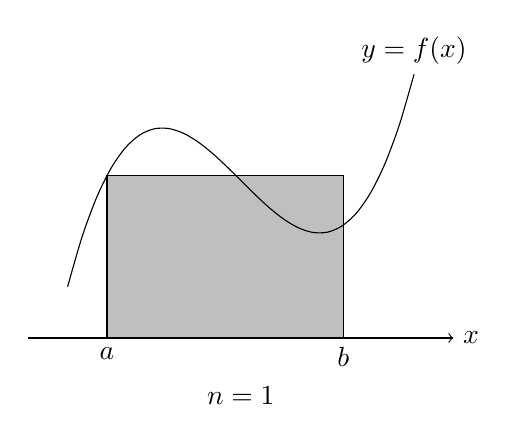
\begin{tikzpicture}[baseline=40] %n=1
	\newcommand{\n}{1}
	\newcommand{\A}{-1.7}
	\newcommand{\B}{1.3}
	\coordinate[label=below:$a$] (a) at (\A,0); %a
	\coordinate[label=below:$b$] (b) at (\B,0); %b
	\foreach \x in {0,...,0}{ %区分和
		\filldraw[fill=lightgray] ($(a)+{\x}*(${1/\n}*($(b)-(a)$)$)$)
		|- ($(a)+{\x+1}*(${1/\n}*($(b)-(a)$)$)+(0,{ (pow(\A+\x/\n*(\B-\A),3)-3*(\A+\x/\n*(\B-\A)))/3+2 })$)
		-- ($(a)+{\x+1}*(${1/\n}*($(b)-(a)$)$)$);
	}
	\draw[->] (-2.7,0) -- (2.7,0) node[right]{$x$}; %x軸
	\draw[smooth,domain=-2.2:2.2] plot(\x, { (pow(\x,3)-3*\x)/3+2 }) node[above] {$y=f(x)$}; %f(x)
	\draw ($(-2.7,-0.5)!0.5!(2.7,-0.5)$) node[below] {$n=\n$};
\end{tikzpicture}
\longrightarrow
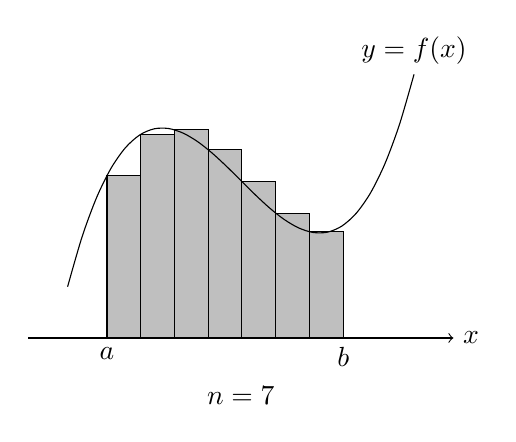
\begin{tikzpicture}[baseline=40] %n=7
	\newcommand{\n}{7}
	\newcommand{\A}{-1.7}
	\newcommand{\B}{1.3}
	\coordinate[label=below:$a$] (a) at (-1.7,0); %a
	\coordinate[label=below:$b$] (b) at (1.3,0); %b
	\foreach \x in {0,...,6}{ %区分和
		\filldraw[fill=lightgray] ($(a)+{\x}*(${1/\n}*($(b)-(a)$)$)$)
		|- ($(a)+{\x+1}*(${1/\n}*($(b)-(a)$)$)+(0,{ (pow(\A+\x/\n*(\B-\A),3)-3*(\A+\x/\n*(\B-\A)))/3+2 })$)
		-- ($(a)+{\x+1}*(${1/\n}*($(b)-(a)$)$)$);
	}
	\draw[->] (-2.7,0) -- (2.7,0) node[right]{$x$}; %x軸
	\draw[smooth,domain=-2.2:2.2] plot(\x, { (pow(\x,3)-3*\x)/3+2 }) node[above] {$y=f(x)$}; %f(x)
	\draw ($(-2.7,-0.5)!0.5!(2.7,-0.5)$) node[below] {$n=\n$};
\end{tikzpicture}\\
\longrightarrow
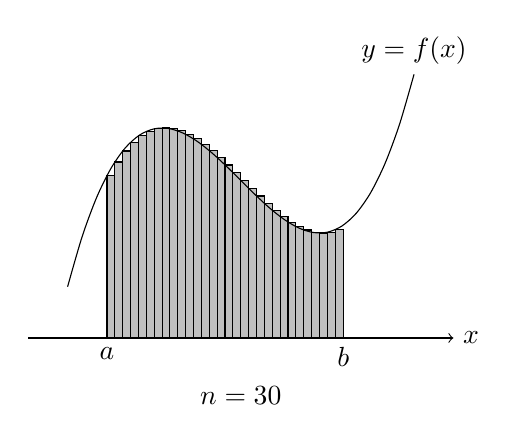
\begin{tikzpicture}[baseline=40] %n=30
	\newcommand{\n}{30}
	\newcommand{\A}{-1.7}
	\newcommand{\B}{1.3}
	\coordinate[label=below:$a$] (a) at (-1.7,0); %a
	\coordinate[label=below:$b$] (b) at (1.3,0); %b
	\foreach \x in {0,...,29}{ %区分和
		\filldraw[fill=lightgray] ($(a)+{\x}*(${1/\n}*($(b)-(a)$)$)$)
		|- ($(a)+{\x+1}*(${1/\n}*($(b)-(a)$)$)+(0,{ (pow(\A+\x/\n*(\B-\A),3)-3*(\A+\x/\n*(\B-\A)))/3+2 })$)
		-- ($(a)+{\x+1}*(${1/\n}*($(b)-(a)$)$)$);
	}
	\draw[->] (-2.7,0) -- (2.7,0) node[right]{$x$}; %x軸
	\draw[smooth,domain=-2.2:2.2] plot(\x, { (pow(\x,3)-3*\x)/3+2 }) node[above] {$y=f(x)$}; %f(x)
	\draw ($(-2.7,-0.5)!0.5!(2.7,-0.5)$) node[below] {$n=\n$};
\end{tikzpicture}
\xrightarrow{\text{定理\ref{thm:quadrature_by_pts}}}
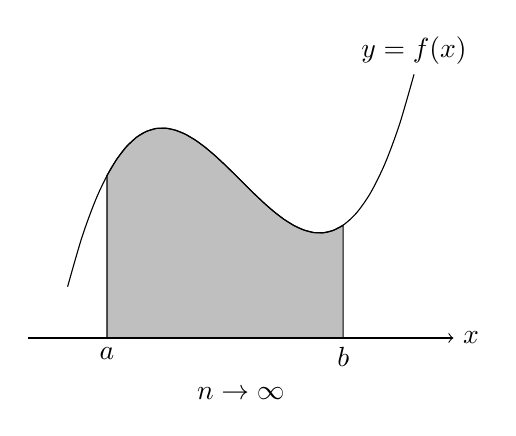
\begin{tikzpicture}[baseline=40] %n=infty
	\newcommand{\A}{-1.7}
	\newcommand{\B}{1.3}
	\coordinate[label=below:$a$] (a) at (-1.7,0); %a
	\coordinate[label=below:$b$] (b) at (1.3,0); %b
	\filldraw[fill=lightgray] (a) -- plot[domain=\A:\B](\x,{(pow(\x,3)-3*\x)/3+2}) -- (b);
	\draw[->] (-2.7,0) -- (2.7,0) node[right]{$x$}; %x軸
	\draw[smooth,domain=-2.2:2.2] plot(\x, { (pow(\x,3)-3*\x)/3+2 }) node[above] {$y=f(x)$}; %f(x)
	\draw ($(-2.7,-0.5)!0.5!(2.7,-0.5)$) node[below] {$n\to\infty$};
\end{tikzpicture}
\end{align*}

\section{補足}

添え字が少し変わった形の等式
\begin{equation}\label{eq:Quadrature_by_pts_2}
	\lim_{n\to \infty}\sum_{k=1}^{n}f(a+k\Delta_n )\Delta_n=\int_{a}^b f(x)\,dx
\end{equation}
も同様に成り立つ.
これは,図形の近似において,各小区間の長方形の高さを右端の値に取ることで得られるが,定理\ref{thm:quadrature_by_pts}から式変形により得ることもできる.

$f(x)$を定理\ref{thm:quadrature_by_pts}の条件を満たす関数とする.
このとき,関数$f(-x)$は区間$[-b,-a]$で連続である.
よって,区分求積法から
\begin{equation*}
	\lim_{n\to \infty}\sum_{k=0}^{n-1}f(-(-b+k\Delta_n ))\Delta_n=\int_{-b}^{-a}f(-x)\,dx
\end{equation*}
が分かる.
右辺は置換積分より$\displaystyle\int_{a}^{b}f(x)\,dx$と等しい.
左辺について,集合の等式
\begin{equation*}
	\{\,b-k\Delta_n\mid k=0,1,\dotsc,n-1\}=\{a+k\Delta_n\mid k=1,2,\dotsc,n\}
\end{equation*}
より
\begin{equation*}
	\sum_{k=0}^{n-1}f(-(-b+k\Delta_n ))\Delta_n=\sum_{k=1}^{n}f(a+k\Delta_n )\Delta_n
\end{equation*}
が成り立つので,\eqref{eq:Quadrature_by_pts_2}が成り立つ.
\end{document}